\documentclass{article}

\usepackage[margin=1in]{geometry}
\usepackage{amsmath}
\usepackage{graphicx}  % needed for figures

\title{Formalizing the ATM problem}
\author{Bryan O'Gorman, Tobias Stollenwerk}
\date{\today}

\begin{document}
\maketitle

These notes attempt to formalize the ATM problem: given a set of flights, schedule them in a way that minimizes cost.
\footnote{It remains to be proven that this problem is hard, either in general or for realistic values of its parameters, e.g. cost functions.}

\section{Configuration space}

At the highest level, the configuration space is a set of 4D trajectories, one for each flight.
By flight we mean an ideal trajectory (times and spatial points) between a 
departure city and arrival city, including an ideal departure time.
Even with relatively coarsely discretized spacetime, that space is infeasably large.
Therefore we parameterize each trajectory by its deviations from the ideal, conflict-ignorant one.
Such deviations are of two types: temporal and spatial. 
A temporal deviation is simply a delayed start (typically on the order of up to 30 minutes). 
We assume that within the time-scale of such delays, the ideal conflict-ignorant trajectory is time-independent.
We consider local spatial deviations, which consist of a set of
maneuvers that change relatively small parts of the spatial trajectory
\footnote{ There could also be global 
spatial deviations, which change the entire trajectory, such as are
used in Olga's thesis.
For example, one parameterization of global spatial deviations treats each
trajectory as an arc in a plane perpendicular to the ground and considers
smooth one-parameter curves to the projection of the trajectory onto the
ground.}.  
Such maneuvers may
introduce a delay, but, as with the delays due to temporal
deviations, we assume that the subsequent ideal trajectory is unaffected 
other than simply being delayed.

Henceforth, we focus on origination delays (temporal deviations) and maneuvers (local spatial deviations).
We assign an index to each flight
\begin{equation*}
    i \in \{i, \dots, n\}
\end{equation*}
For each flight $i$, the wind-optimal trajectories are given as a sequence of $M_i$ 4-dimensional space-time points
\begin{equation*}
    \tau_i = \{p^i_1, \dots, p^i_{M_i}\}
\end{equation*}
with
\begin{equation*}
    p^i_j = \left( \varphi^i_j, \lambda^i_j, z^i_j, t^i_j \right)
\end{equation*}
where $(\varphi^i_j, \lambda^i_j)$ are the latitude and longitude.
For simplicity, we will assume a constant altitude $z^i_j$ for all flights.
\begin{equation*}
    p^i_j = \left( \varphi^i_j, \lambda^i_j, t^i_j \right)
\end{equation*}

\section{Potential conflicts}
Conflicts may occur if multiple flight trajectories
\begin{equation*}
    \{\tau_i : i \in I_k \subseteq \{1, \dots, n\}\}
\end{equation*}
become too close to each other in time and space.

In the following we will define spatial, potential, and real conflicts.
A \textit{spatial conflict} occurs if two trajectories become too close 
to each other in space.
The existence of a \textit{real conflict} depends on the arrival time of both flights and at the spatial conflict.
A \textit{potential conflict} exists, if a real conflict is possible considering a maximal flight delays upon arrival at the spatial conflict.
For details, see appendix \ref{app:potential_conflicts}.

In any case, we index the potential conflicts by $k$.
A classical precalculation gives us the mapping to the involved flights
\begin{equation*}
    k \mapsto I_k \subseteq \{1, \dots, n\}\}
\end{equation*}
as well as the set of conflicts the flight $i$ is involved in
\begin{equation}
    i \mapsto \{k^i_1, \dots, k^i_{N_i}\} =: K_i
\end{equation}
Moreover, we can order the $N_i$ conflicts the flight $i$ is involved in by their temporal appearance:
\begin{equation*}
    i \mapsto (k^i_1, \dots, k^i_{N_i})
\end{equation*}
In the following it will prove useful to introduce the set of conflicts the flight $i$ was involved in before it arrives at a potential conflict $k$
\begin{equation*}
    K^<_{ik} = \{\tilde k : \tilde k \in\{k^i_0, \dots, k^i_{N_i}\}, \tilde k < k\}
\end{equation*}
Note that the conflicts may note be point conflicts, but may extend in time ans space. See the appendix.


\section{Cost function}
In reality, the cost function results from factors such as fuel, labor, time, etc.; here we treat it as a unitless quantity that appropriately weights these factors.
Because we are interested in the relative costs of different configurations, we treat the cost of the configuration in which all flights are routed along their independently optimal trajectories, ignoring conflicts, and are exactly on time, as zero.
We further assume that the total cost is the sum of two different types of costs:
\begin{itemize}
  \item for each flight $i$, the cost $c_i^{\mathrm{late}}$ of being late on arrival,
  \item for every conflict $k$, the cost $c_k^{\mathrm{avoid}}$ of avoiding it.
\end{itemize}
The total cost therefore is 
\begin{equation*}
c = 
\sum_i c^{\mathrm{late}}_i + 
\sum_{k} c^{\mathrm{avoid}}_k
,
\end{equation*}
where each contribution to the cost function depends (implicitly as written so far) on the configuration space.
Because the lateness and avoidance costs are associated with flights and conflicts, respectively, we write simply $c_i = c_i^{\mathrm{late}}$ and $c_{k} = c_{k}^{\mathrm{avoid}}$ where the distinction is clear from context.
Henceforth, we simplify things by ignoring the direct cost of the local maneuvers. 
However, they will still indirectly contribute to the cost function via their introduction of delays.
The quantity to minimized can then be written
\begin{equation*}
c = 
\sum_i c_i (D_i),
\end{equation*}
where $D_i = d_i + \sum_{K_i} d_{ik}$ is the delay of flight $i$ at its destination, which will be a function of its origination delay $d_i$ and delays $\{d_{ik}\}$ introduced by avoiding the potential conflict $k$ by a local maneuvers.

Lastly, we simplify things further by assuming that all destination delays are equally important, (which comes by necessity from the absence of information to the contrary), so that the quantity to minimize is simply the total delay of all flights:
\footnote{The lack of information with respect to the relative importance of flights in reality only requires that all $c_i$ be the same function. One could imagine minimizing the $L_2$ norm(which would help avoid having a few very late flights) rather than the $L_1$ norm as we do here, or indeed any other function. The simple sum here is the one currently used by Olga et al., and has the advantage of being most conducive to mapping to QUBO.}
\begin{equation} \label{eqn:total_delay}
c = D = \sum_i D_i.
\end{equation}


\section{Classical precalculation}
\label{sec:classical_precalculation}
We assume the availability of the following classical routines, whose resource requirements we regard as negligible:
\begin{itemize}
\item Given the trajectories of all flights, return the potential conflicts
    \begin{equation*}
        \{\tau_1, \dots, \tau_n\} \mapsto \{k_1, \dots, k_m\}
    \end{equation*}
    and the corresponding parameters attached to a potential conflict $k$:
    \begin{itemize}
        \item The set of involved flights $I_k$
        \item The trajectory points involved $\{p^i_j : j\in J \subseteq M_i,  i \in I_k,\}$
    \end{itemize}
\item Given the above potential conflict parameter, return the delays introduced by a conflict avoiding maneuver
    \begin{equation*}
        k \mapsto d_{ik} \quad \forall i \in I_k 
    \end{equation*}
    This delay may depend on a set of maneuver parameters. 
    \begin{equation*}
        \mathbf{a_k} =  (a^1_k, \dots, a^{L_k}_k)
    \end{equation*}
\end{itemize}

\section{Assumptions made}
\begin{itemize}
\item For each flight, the optimal route is time-independent (both spatially and in duration) over the timescale of possible delays.
For example, if the flight has no potential collisions, its lateness on arrival will exactly equal its departure delay.
\item Actively avoiding a collision (rather than avoiding via departure delays) does not change the cost of actively avoiding other collisions on the same flight path. In reality, one could reason, e.g. that the little bit of fuel used in each active collision avoidance could add up to a disastrously empty tank, but in general we would like the effect of active collision avoidances to be as little as possible.
Similarly, one could argue that the plane burns fuel while idling.
\end{itemize}

\section{Potentially helpful assumptions}
\begin{itemize}
\item (Sparseness) All conflicts are pairwise. That is, when two planes have a potential conflict, there are no other planes nearby. 
Furthermore, when this conflict is avoided, it does not create a conflict with another flight. 
(This may be the most unreasonable assumption, e.g. near major airports or on crowded jetstreams.)
\item Collisions are symmetric. That is, the cost of avoiding them is a function only of the magnitude of the difference in delays of the two flights up until that point. For example, the cost of avoiding a collision between $i$ and $j$ is the same whether $i$ is delayed by $d$ or $j$ is.
\item The lateness cost functions are non-decreasing.
% we might as well allow it to be negative for earliness, though that could be
% compiled away by pushing the range of available departure times earlier. 
This is obviously satisfied for the linear cost functions with unit slope used
here, and hard to imagine relaxing.
\end{itemize}

\section{Models}
\label{sec:models}
The arrival time of flight $i$ at a potential conflict $k$ reads 
\begin{equation*}
    T_{ik} = t_{ik} + d_i + \sum_{p \in K^<_{ik}} d_{ip}
\end{equation*}
where $t_{ik}$ is the arrival time in the wind-optimal case.
The delay it has picked up upon arrival at the potential conflict $k$, is
\begin{align*}
    D_{ik} &= T_{ik} - t_{ik} \\
           &= d_i + \sum_{p \in K^<_{ik}} d_{ip}
\end{align*}

\subsection{General Model}
In general, the delay introduced by conflict avoiding maneuver $d_{ik}$ is a
function of the arrival delay of each involved flight $D_{jk}, \forall j \in
I_k$ and the maneuver parameters $\mathbf{a_k}$ \begin{equation}
\label{eqn:local_delay}
    d_{ik} = d_{ik}(\mathbf D_{k}, \mathbf{a_k}) 
\end{equation}
where $\mathbf D_k = (D_{jk})_{j \in I_k}$.
This function is given as a classical routine mentioned in section \ref{sec:classical_precalculation}.
The total delay \eqref{eqn:total_delay} is then given by
\begin{align*}
    D &= \sum_i \left(d_i + \sum_{k\in K_i} d_{ik}\right) \\
      &= \sum_i \left(d_i + \sum_{k\in K_i} d_{ik}(\mathbf D_{k}, \mathbf{a_k})\right) \\
\end{align*}

\subsection{Sparse case}
First, we describe a method for solving the ``sparse'' version of the problem.
By sparsity, we mean that all potential conflicts are between only two
trajectories and that no other trajectories are nearby in spacetime, so that
potential maneuvers for avoiding a conflict between two flights do not
introduce additional potential conflicts with other flights.\footnote{This
could be extended to an $m$-sparse version, where each conflict can affect
$m-1$ others.}

Making the assumption that the maneuvers depend only on the difference
between of the arrival times of the flights, 
we can write $d_{ik}$ as a function of the difference of the delays 
for the two flights, where $i$ can be either of the two indices $j$ and $l$, 
with $l<j$, involved in conflict $k$.
\begin{equation*}
    \Delta_{k} := D_{lk} - D_{jk} \quad l < j \in I_k
\end{equation*}
and the maneuver parameters $\mathbf{a}_k$.
It's plausible to assume that it furthermore depends only on the magnitude of this difference $|D_{lk} - D_{jk}|$, though it's not yet clear that that will help.
With this \eqref{eqn:local_delay} becomes
\begin{equation*}
    d_{ik} = d_{ik}(\Delta_{k}, \mathbf{a}_k) 
\end{equation*}
and the total delay reads
\begin{equation*}
    D = \sum_i \left(d_i + \sum_{k\in K_i} d_{ik} (\Delta_k, \mathbf{a}_k)\right).
\end{equation*}
Three special cases are as follows. 

\subsubsection{No Delay Model}

In the (totally unrealistic) case where maneuvers do not introduce any further delays, we have simply
\begin{equation*}
    \Delta_k = d_i - d_j
\end{equation*}
and 
\begin{align*}
    d_{ik} &= d_{ik}(d_l, d_j) \quad (l, j) \in I_k \\
           &= 
            \begin{cases} 
                0,      & \text{potential conflict $k$ can be avoided given delays $d_l$ and $d_j$, $(l, j) \in I_k$}\\
                \infty, & \text{otherwise}.
            \end{cases}
\end{align*}
For the assumption that maneuvers do not introduce further delays to make any sense at all, we must bound their size, which is why some conflicts simply cannot be avoided within this approximation.
Of course, we define $d_{ik}$ as piece-wise infinite for consistency with the rest of these notes, but in practice this would be implemented as a hard constraint.
(Interestingly, this notational device has the morose interpretation that if the flights do collide, the further delay introduced is indeed infinite.)

\subsubsection{Independent Delay Model}
In this model we assume that the delay introduced by a conflict-avoiding 
maneuver is independent of the other flight. 
% There are no spatial maneuvers, but each flight $i$ is allowed to slow down by
% some delay $d_{ik}$ before conflict $k$ (and after the its previous one).  
%In the above formalism, this is equivalent to $\mathbf a_k = (d_{ik}, d_{jk})$.
%In this case, there is no need for $\left(d_i\right)_{i=1}^n$ because for each flight the origination delay $d_i$ can just be subsumed into the delay $d_{ik}$ of the first conflict.
Each potential conflict $k$ is an actual conflict when the difference between the total delays of the constituent flights are in some range $\left[\Delta_k^{\mathrm{min}}, \Delta_k^{\mathrm{max}}\right]$.
However, it is not clear how to penalize real conflicts.

\subsubsection{Delay Frontier Model}
For a given $\Delta_{k}$ and $(l, k) \in I_k$ we assume that there is a minimal delay of each flight $d_{lk}^*$ and $d_{jk}^*$ assuming that the other is unchanged, and there is (presumably) a concave ``delay frontier'' in the region $[0, d_{lk}^*] \times [0, d_{jk}^*]$ connecting $(d_{lk}^*, 0)$ and $(0, d_{jk}^*)$ that gives the possible delays $(d_{lk}, d_{jk})$. 
We parameterize this curve by the scalar $a_{k} \in [0, 1]$.
More generally, there is a ``delay surface'' when various values of $\Delta_{k}$ are considered.
Discretizing $a_k$ into only two values $\{0, 1\}$ is equivalent to requiring that exactly one flight maneuvers around the other, whose trajectory remains unchanged.

In order to formulate the problem as a QUBO, we discretize and introduce bits for each discrete value for the variables $d_i$, $d_{ik}$, $\Delta_k = D_{lk} - D_{jk}$, and $a_k$:
\begin{equation*}
    C = D + p_1 C^{\mathrm{one}} + p_2 C^{\mathrm{equal}},
\end{equation*}
where 
\begin{equation*}
D = 
\sum_{i} \sum_{\alpha} \alpha d_{i\alpha}
+
\sum_{ik} \sum_{\beta} \beta d_{ik\beta}
\end{equation*}
is the delay to be minimized,
\begin{equation*}
C^{\mathrm{one}}
=
\sum_i \left(\sum_{\alpha} d_{i\alpha}- 1 \right)^2 
+
\sum_{ik} \left(\sum_{\beta} d_{ik\beta} - 1\right)^2
+
\sum_{k} \left(\sum_{\gamma} \Delta_{k\gamma} - 1\right)^2
+
\sum_{k} \left(\sum_{\delta} a_{k\delta}- 1\right)^2
\end{equation*}
is the penalty function ensuring that each variable has a well defined value encoded by a single bit,
\begin{align*}
C^{\mathrm{equal}}
&=
\sum_{k} \left[
\left(\sum_{\alpha} \alpha d_{l\alpha} + \sum_{p \in K^<_{lk}} \sum_{\beta} \beta d_{lp\beta}\right)
-
\left(\sum_{\alpha} \alpha d_{j\alpha} + \sum_{q \in K^<_{jk}} \sum_{\beta} \beta d_{jq\beta}\right)
-
\left(\sum_{\gamma} \gamma \Delta_{k\gamma}\right)\right]_{(l, j) \in I_k }^2
+ \\
&\hphantom{=,}
\sum_{ik} \left[
    \left(\sum_{\beta} \beta d_{ik\beta}\right) - 
\left(\sum_{\gamma \delta} d_{ik} (\gamma, \delta) \Delta_{k\gamma} a_{k\delta}\right)\right]^2
\end{align*}
is the penalty function ensuring that $\Delta_k = D_{ik} - D_{jk}$ and $d_{ik} = d_{ik}(\Delta_k, a_k)$, 
the Greek indices represent the discrete values that the corresponding quantities can assume, and $p_1$ and $p_2$ are penalty weights.\footnote{In practice we could have varying penalty weights for the various penalties.}
Note, that the last term introduces cubic and quartic terms.

We could make a further approximation and for each conflict pick some optimal-in-expectation $a_k$, thereby removing that variable from the formulation.
This would decrease the degree of the above cost function resulting in a QUBO.
Alternatively, we could allow the delays $(d_{ik}, d_{jk})$ to take on any value at or beyond the delay frontier (i.e. somewhere in between the independent delays and delay frontier cases).
We could also suitably parameterize the ``delay surface'' so that the cost function could be written in a functional form.

\subsubsection{Variations of the Delay frontier model}
We can reduce the number of variables by
\begin{enumerate}
    \item Both flights will always \textit{split the delay}: Set $a_k$ to a fixed value inside $[0, 1]$, presumably $a_k = 0.5$. This would eliminate all variables $a_{k\beta}$.
    \item One flight makes a detour, the other remains on the wind-optimal route: Reduce the possible values values of $a_k$ to either $0$ or $1$. Hence $a_k$ itself becomes a binary variable.
\end{enumerate}

\subsection{Dense case}
The sparsity condition assumed above is in general false, even when ignoring near-airport trajectories.
The other extreme is the ``dense'' case, in which all flights are restricted to a ``highway'' as in Olga's thesis.
An appropriate QUBO for that problem is relatively straightforward, and can be written explicitly if needed.

\subsection{General case}
General instances fall into neither of the above extremes.
One potential solution is to use some sort of master-slave subproblem decomposition to combine solvers for each extremal case into a general solution.

\section{Mapping to Job Shop Scheduling}
We can map the ATM problem to job shop scheduling by imagining the space at a potential conflict $k$ as a resource, the flights $I_k$ have to compete for.
\begin{equation*}
    R_k = \text{spatial trajectory points of the flights } i \in I_k \text{which are in (spatial) conflict with each other}
\end{equation*}
In the language of job shop scheduling, we have a ordered set of tasks for each flight $i \in I_k$:
\begin{equation*}
    \mathcal{T}_i = \left(R^{t_0}_i, \dots, R^{t_M}_i\right)
\end{equation*}
where $t_0$ and $t_M$ are the earliest and the latest time in the whole trajectory data set.
$R^t_i$ is the resource assigned to flight $i$ at time $t$.
If a flight $i$ at time $t'$ occupies a spatial trajectory point which is not in spatial conflict with any other flight, it is viewed as using the resource $R_i$, i.e.\ $R^{t'}_i = R_i$.
The role of conflict avoiding maneuvers is replaced by the a task waiting for a resource occupied by a conflicting flight to free up.
\subsection{Example}
Assume three flights and two potential conflicts between flight $1$ and $2$ as well as between $2$ and $3$ (see figure \ref{fig:jobshop_example}).
Let the set of tasks for each flights read
\begin{align*}
    \mathcal{T}_1 &= \left(R_1, R_1, R_{k_1}, R_1, R_1\;\,, R_{k_2}, R_1\right) \\
    \mathcal{T}_2 &= \left(R_2, R_2, R_{k_1}, R_2, R_2\;\,, R_2\;\,, R_2 \right) \\
    \mathcal{T}_2 &= \left(R_3, R_3, R_3\;\,, R_3, R_{k_2}, R_3\;\,, R_3 \right) 
\end{align*}

\begin{figure}[htpb]
    \centering
    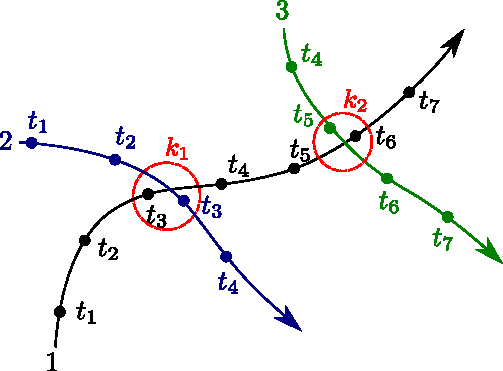
\includegraphics[width=0.6\linewidth]{pics/jobshop_example}
    \caption{Example for mapping to job shop scheduling}
    \label{fig:jobshop_example}
\end{figure}

\newpage
\appendix
\section{Potential conflicts}
\label{app:potential_conflicts}
\subsection{Spatial conflicts}
In the following we will restrict ourselves to pairwise conflicts.
Given a spatial conflict between the flights $i$ and $j$, a real conflict exists if the arrival times at the spatial conflict $k$, $T_{ik}$ and $T_{jk}$ (see figure~\ref{fig:spatial_conflicts}) obey certain conditions.
The corresponding departure times from the spatial conflict are denoted by 
\begin{equation*}
    T'_{ik} = \frac{L_k}{v_i} + T_{ik}
\end{equation*}
where $L_k$ spatial length of the spatial conflict $k$ and $v_i$ is the constant velocity of flight $i$.
\begin{figure}[htpb]
    \centering
    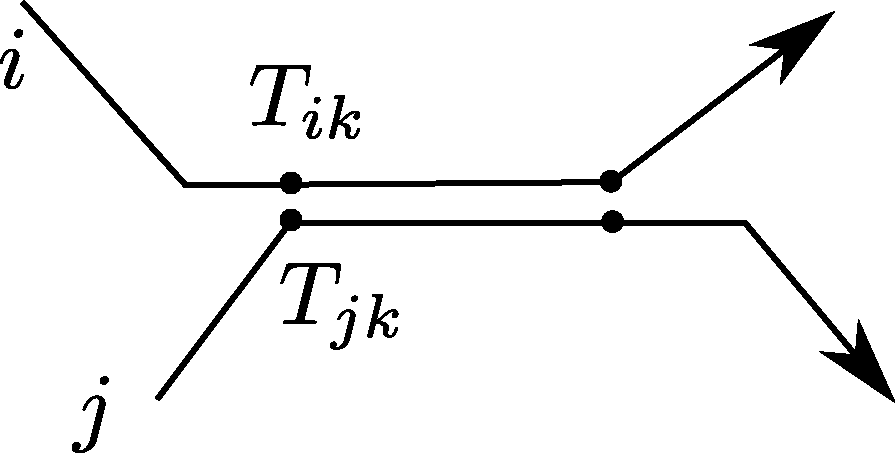
\includegraphics[width=0.3\linewidth]{pics/spatial_conflict_parallel.pdf}
    \hspace{1cm}
    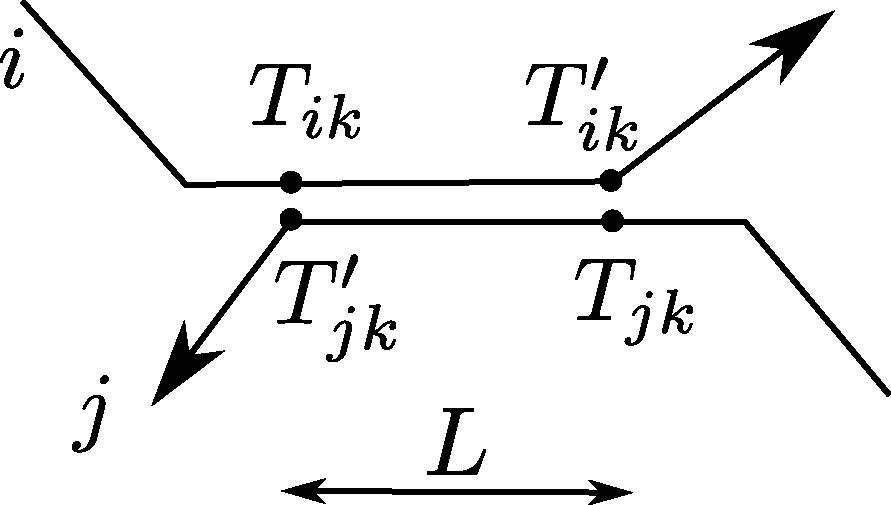
\includegraphics[width=0.3\linewidth]{pics/spatial_conflict_anti_parallel.pdf}
    \caption{Parallel and antiparallel spatial conflict}
    \label{fig:spatial_conflicts}
\end{figure}

\begin{itemize}
    \item {\bf Parallel conflict:}
        A real conflict exists if the difference between the arrival times is smaller than a threshold $\Delta_p$ which depends on the trajectories, in particular the speed and position of both flights.
        \begin{equation*}
            \bigl| \underbrace{T_{jk} - T_{ik}}_{\Delta_k} \bigr| < \Delta_p
        \end{equation*}
        with
        \begin{equation*}
            \Delta_p = \Delta_p(v_i, v_j, r_i, r_j)
        \end{equation*}
        This can also be written as
        \begin{equation}  \label{eqn:conflict_parallel}
            -\Delta_p < \Delta_k < \Delta_p 
        \end{equation}
        
    \item {\bf Antiparallel conflict:}
        A real conflict exists if 
        \begin{equation*}
            T'_{ik} - T_{jk} < \Delta^1_{ap}(v_i, v_j, r_i, r_j)
        \end{equation*}
        and
        \begin{equation*}
            T'_{jk} - T_{ik} < \Delta^2_{ap}(v_i, v_j, r_i, r_j)
        \end{equation*}
        Hence
        \begin{eqnarray*}
            \frac{L_k}{v_i} + \underbrace{T_{ik} - T_{jk}}_{-\Delta_k} < \Delta^1_{ap} \\
            \frac{L_k}{v_j} + \underbrace{T_{jk} - T_{ik}}_{\Delta_k} < \Delta^1_{ap} 
        \end{eqnarray*}
        This yields
        \begin{equation} \label{eqn:conflict_antiparallel}
            \frac{L_k}{v_i} - \Delta^1_{ap} < \Delta_k < \Delta^2_{ap} - \frac{L_k}{v_j}
        \end{equation}
\end{itemize}

\subsection{Potential conflicts}
The arrival time $T_{ik}$ is given by the arrival time in the wind optimal case $t_{ik}$ plus the delay it picked up due to earlier conflict avoiding maneuvers or a departure delay $D_{ik}$. 
\begin{equation*}
    T_{ik} = t_{ik} + D_{ik} \quad \forall i, k
\end{equation*}
and the difference of the arrival time of the two flights $i$ and $j$ at spatial conflict $k$ is given by
\begin{eqnarray*}
    \Delta_k &=& T_{ik} - T_{jk} \\
             &=& t_{ik} - t_{jk} + D_{ik} - D_{jk}
\end{eqnarray*}
The maximal value of $D_{ik}$, $\forall i, k$ is bounded from above by some $D^{\text{max}}$.
Hence, $\Delta_k$ is bounded by
\begin{equation} \label{eqn:potential_conflict}
    (t_{ik} - t_{jk} - D^{\text{max}})< \; \Delta_k \; < (t_{ik} - t_{jk} + D^{\text{max}})
\end{equation}
Therefore, we identify a spatial conflict $k$ as a \textbf{potential conflict} if for a $\Delta_k$ which is bounded by \eqref{eqn:potential_conflict}, one of the inequalities \eqref{eqn:conflict_parallel} or \eqref{eqn:conflict_antiparallel} is fulfilled.

From now on, all indices $k$ will denote potential conflicts.

\end{document}
